\chapter{SOLID}

\section{Analyse Single-Responsibility-Principle (SRP)}
\subsection{Positiv-Beispiel}
Die nachfolgende Abbildung zeigt das gekürzte UML-Diagramm der Klasse
\textit{CollectAction}. Die ist in der Schicht \textit{plugins}
angesiedelt. Sie implementiert das \textit{IAction}-Interface, welche
vom Spieler initiierte Aktionen darstellt. Die einzige Aufgabe der
\textit{CollectAction} ist es, zu prüfen, ob ein Item unter dem 
Spieler liegt und dieses aufzunehmen bzw. mit dem bisherigen Item
gleichen Typ (z.B. Rüstung) auszutauschen. Dafür bekommt es ein
\textit{Game}-Objekt übergeben, aus welchem die nötigen Informationen
gezogen und die nötigen Funktionen aufgerufen werden können.

\vspace{0.5cm}
\begin{figure}[H]
    \centering
    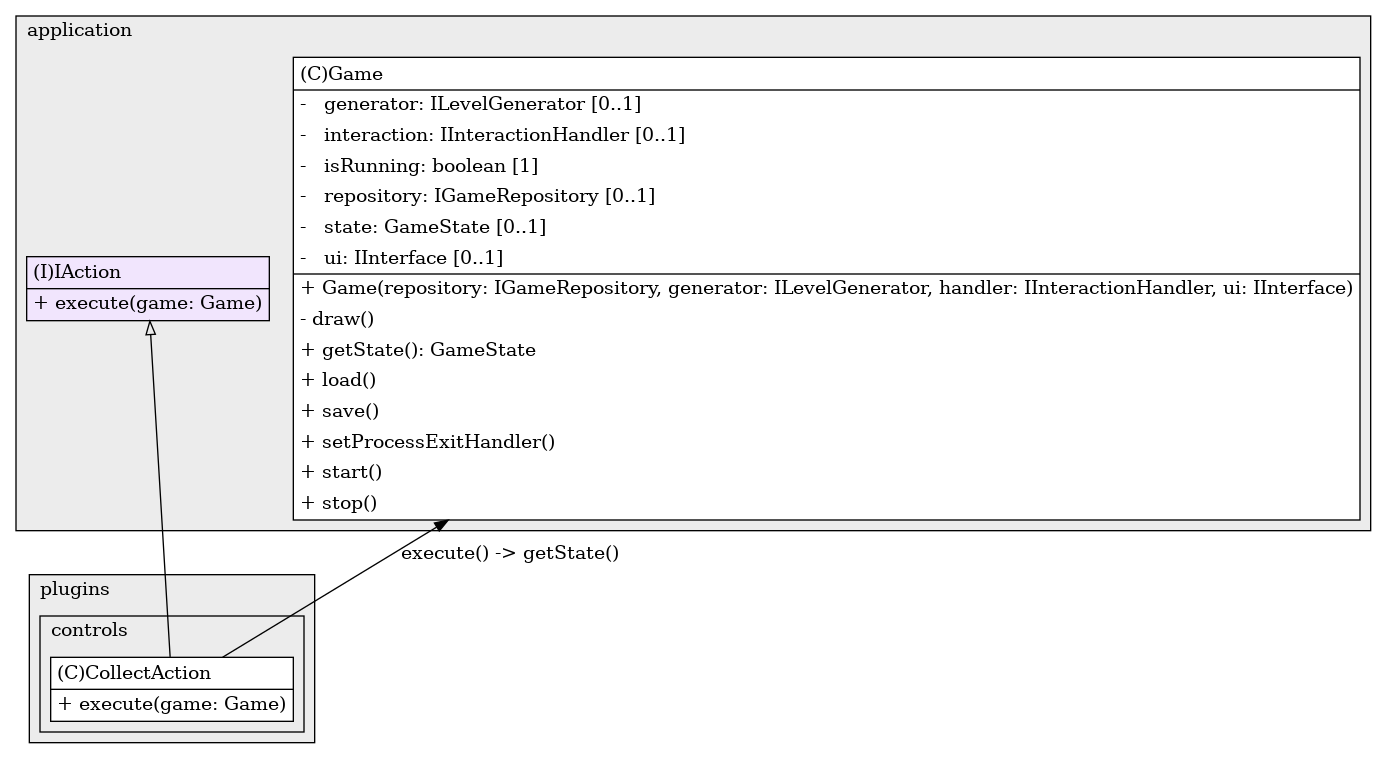
\includegraphics[width=1\linewidth]{Bilder/Visualisierung/CollectActionSimplified_structure.png}
    \caption{Analyse Single-Responsibility-Principle: Positiv}
\end{figure}

\subsection{Negativ-Beispiel}

\section{Analyse Open-Closed-Principle (OCP)}
\subsection{Positiv-Beispiel}
Die nachfolgende Abbildung zeigt das gekürzte UML-Diagramm des Interfaces
\textit{IAction}. Dieses ist in der Schicht \textit{application}
angesiedelt. Die \textit{Main}-Klasse mit ihrem \textit{Game Loop}
kennt lediglich das Aktions-Interface \textit{IAction}. Es bezieht
die Aktionen aus einem \textit{IInteractionHandler} (hier zur
Vereinfachung nicht mit dargestellt). Diese werden dann mittels
ihrer \textit{execute()}-Methode ausgeführt. 

Diese Struktur ermöglicht die Einhaltung des
\textit{Open-Closed-Principles}. Um eine neue Aktion zu implementieren,
muss lediglich eine weitere Klasse hinzugefügt werden, welche das 
\textit{IAction}-Interface implementiert. Alle anderen Implementierungen
des \textit{IAction}-Interface bleiben dabei unberührt, ebenso wie die
\textit{Main}-Klasse.

Die Verwendung dieses Schemas ist sehr sinnvoll, da vor allem in den
frühen Phasen der Spielentwicklung viele Änderungen bezüglich der
Spielerfahrung gemacht werden. Davon sind auch Aktionen und
Tasteneingaben betroffen. Mit dem \textit{IAction}-Interface lassen
sich somit schnell Änderungen mit minimalem Eingriff umsetzen. Es
müssen keine schnell unübersichtlichen \textit{switch}-Statements
benutzt werden. 

\vspace{0.2cm}
\begin{figure}[H]
    \centering
    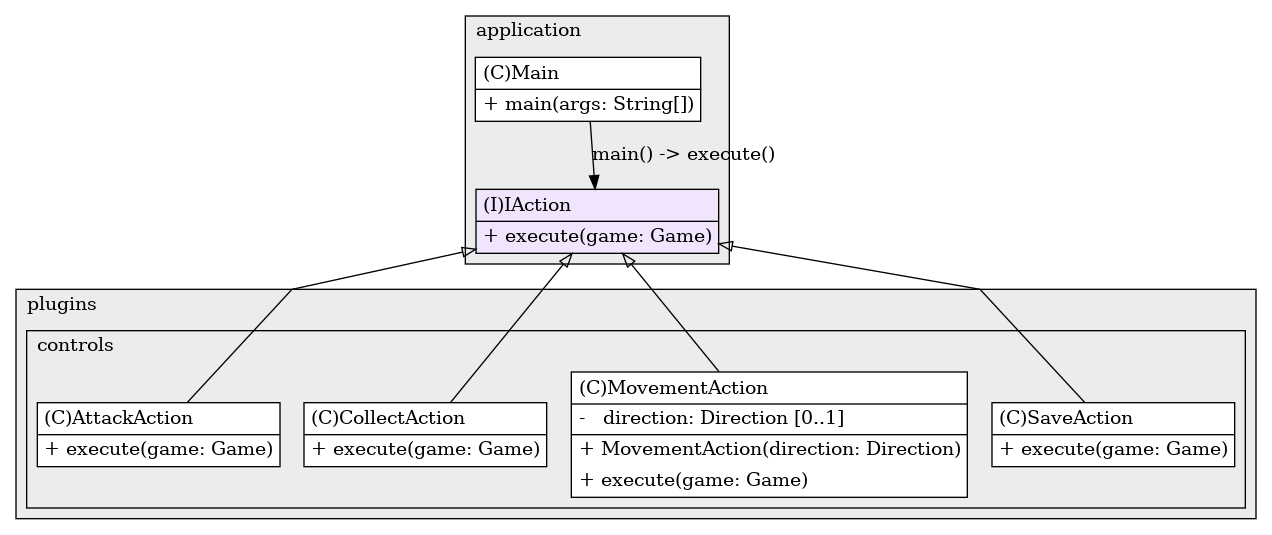
\includegraphics[width=1\linewidth]{Bilder/Visualisierung/IAction_structure.png}
    \caption{Analyse Open-Closed-Principle: Positiv}
\end{figure}

\subsection{Negativ-Beispiel}

\section{Analyse Dependency-Inversion-Principle (DIP)}